\chapter{积分变换法}
\thispagestyle{empty}

\tdefination[积分变换]
把函数$f(t)$经过积分运算变换为另一类函数
\begin{align}
	F(\beta) = \int_a^b f(t)K(\beta, t) \, \d t
\end{align}
其中,
\begin{itemize}
	\item $\beta$为参变量,$K(\beta, t)$为一个确定的二元函数,称为\dy[积分变换的核]{JFBHDH}\vspace*{-0.5em}
	\item 不同的核与不同的积分区域,构成不同的积分变换\vspace*{-0.5em}
	\item 主要包括Fourier变换和Laplace变换
\end{itemize}

\section{Fourier变换}
\vspace{0.5em}
\ttheorem[Fourier变换]
\dy[Fourier变换]{FourierBH}
\begin{align}
	F(\omega) = \mathcal{F}\big[f(x)\big] = \int_{- \infty}^{+ \infty} f(x) \e^{- \i \omega x}\, \d x
\end{align}
\vspace*{-2em}

\dy[反演]{FY}
\begin{align}
	f(x) = \mathcal{F}^{-1} \big[F(\omega)\big] = \dfrac{1}{2 \pi} \int_{- \infty}^{+ \infty} F(\omega) \e^{\i \omega x}\, \d \omega
\end{align}

\warn[
Fourier变换的重要条件:\textbf{分段光滑}\footnote{\textbf{分段光滑}:一阶导数存在,且导函数只有第一类间断点。}、\textbf{绝对可积}$\displaystyle \int_{- \infty }^{+ \infty} \big|f(x)\big|\, \d x < + \infty$\vspace*{-0.5em}
{
\begin{enumerate}[\hspace*{2em} \textbf{推论} 1 \hspace*{2em}]
	\item $\displaystyle \int_{- \infty}^{+ \infty} f(x)\, \d x = \mbox{有限值}$
	\item $x \to \pm \infty, f(x) \to 0$
\end{enumerate}
}
]

\subsection{Fourier变换的理解}
Fourier变换从几何上看是将函数分解成无数个绕原点做圆周运动的向量,得到相位/半径 与频率的函数关系;本质上是分解成无数个不同频率、幅值和相位正弦函数。

物理上认为,$f(x)$为信号(原函数), $F(\omega)$为频谱(像函数),对$f(x)$进行Fourier变换,实际上是由信号得到频谱的过程(从时域到频域),称为\dy[Fourier分析]{FourierFX}。

对于Fourier变换的进一步理解,如图\ref{Fourier变换的理解图}.

\begin{figure}[!htb]
	\centering
	\begin{tikzpicture}
		\node (A) [draw, inner sep = 5pt]{\makecell[c]{周期函数可以表示为不同频率、\\幅值和相位的正弦函数的叠加}};
		\node (B) [draw, inner sep = 5pt, below of = A, node distance = 3.5cm]{\makecell[c]{当函数的周期较小时,正弦函数的频率\\是稀疏的,因此叠加体现为无穷级数}};
		\node (B1) [draw, inner sep = 5pt, right of = B, node distance = 9cm]{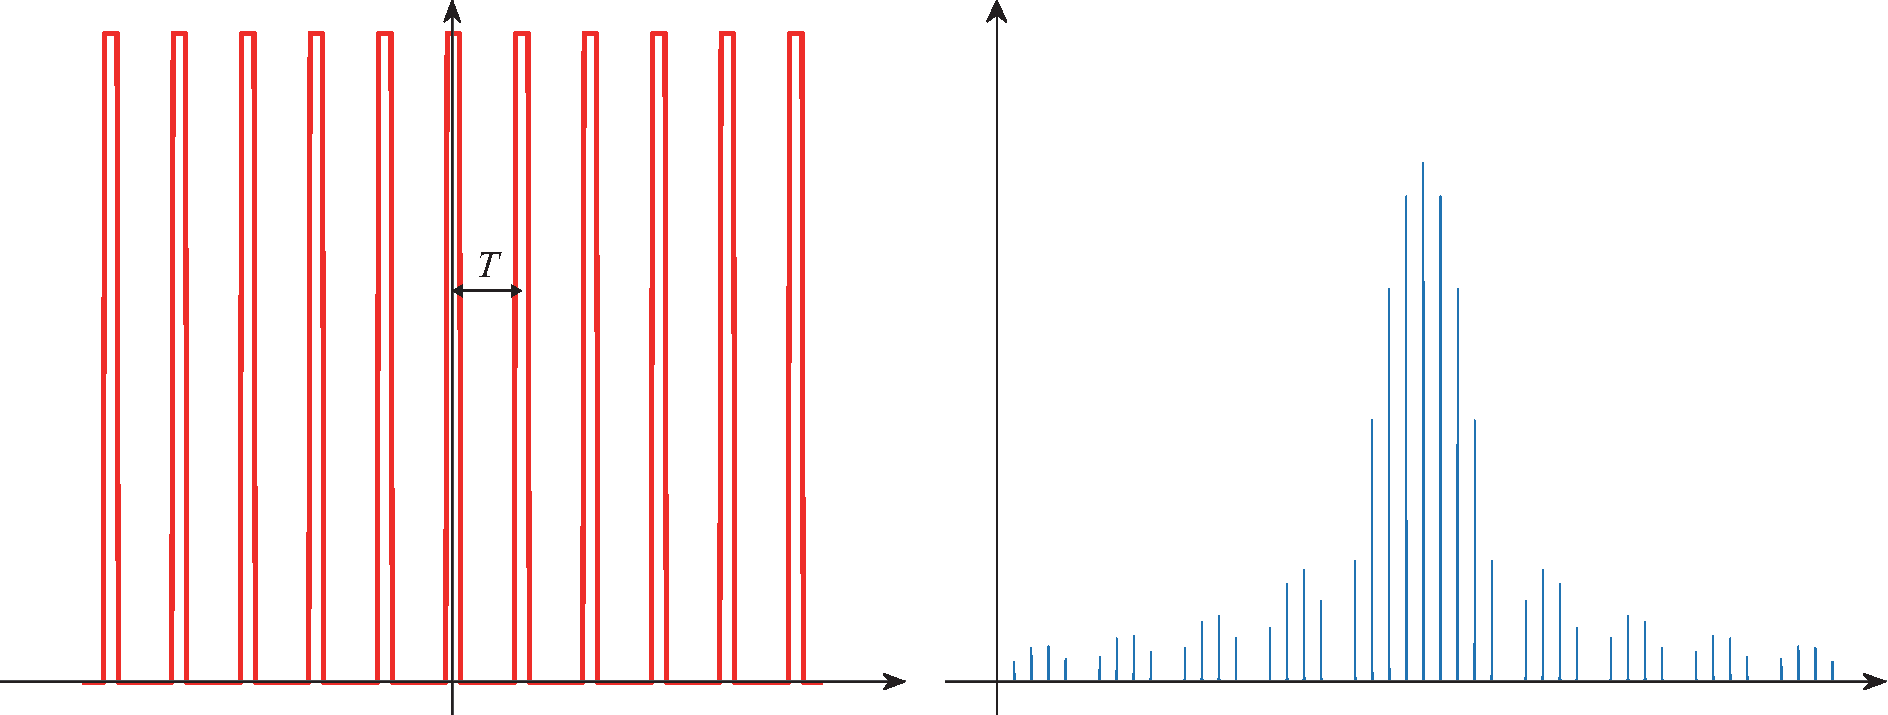
\includegraphics[width=0.5\linewidth]{pic/Fo1.pdf}};
		\node (C) [draw, inner sep = 5pt, below of = B, node distance = 5cm]{\makecell[c]{随着周期的增加,正弦函数的频率\\从稀疏走向密集}};
		\node (C1) [draw, inner sep = 5pt, right of = C, node distance = 9cm]{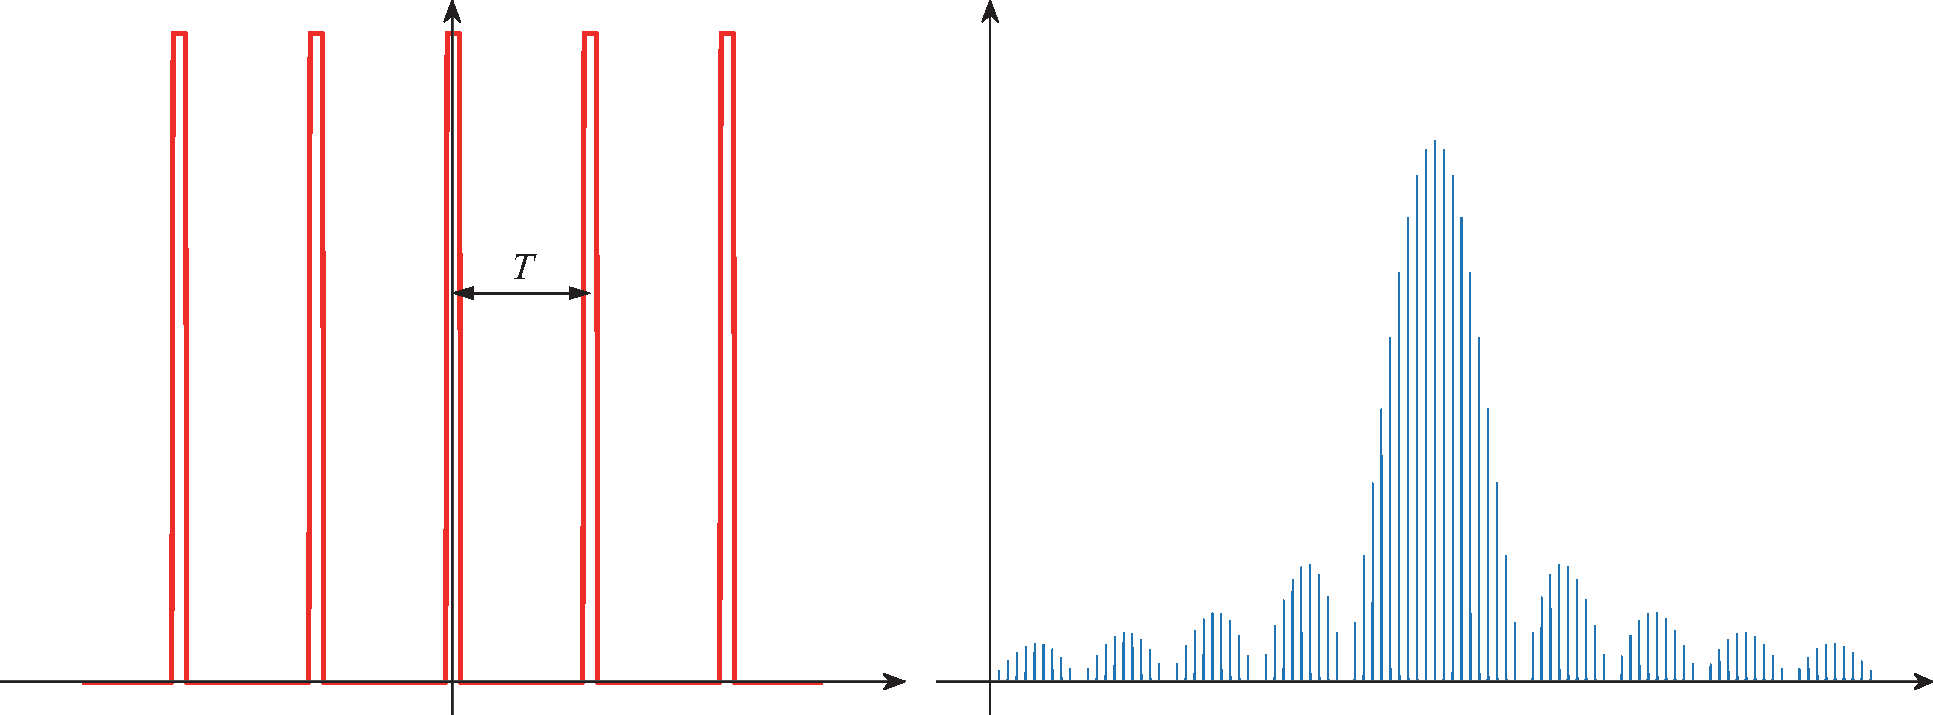
\includegraphics[width=0.5\linewidth]{pic/Fo2.pdf}};
		\node (D) [draw, inner sep = 5pt, below of = C, node distance = 5cm]{\makecell[c]{当周期为无穷大时,正弦函数的频率\\演变为连续的,叠加也由级数变为积分}};
		\node (D1) [draw, inner sep = 5pt, right of = D, node distance = 9cm]{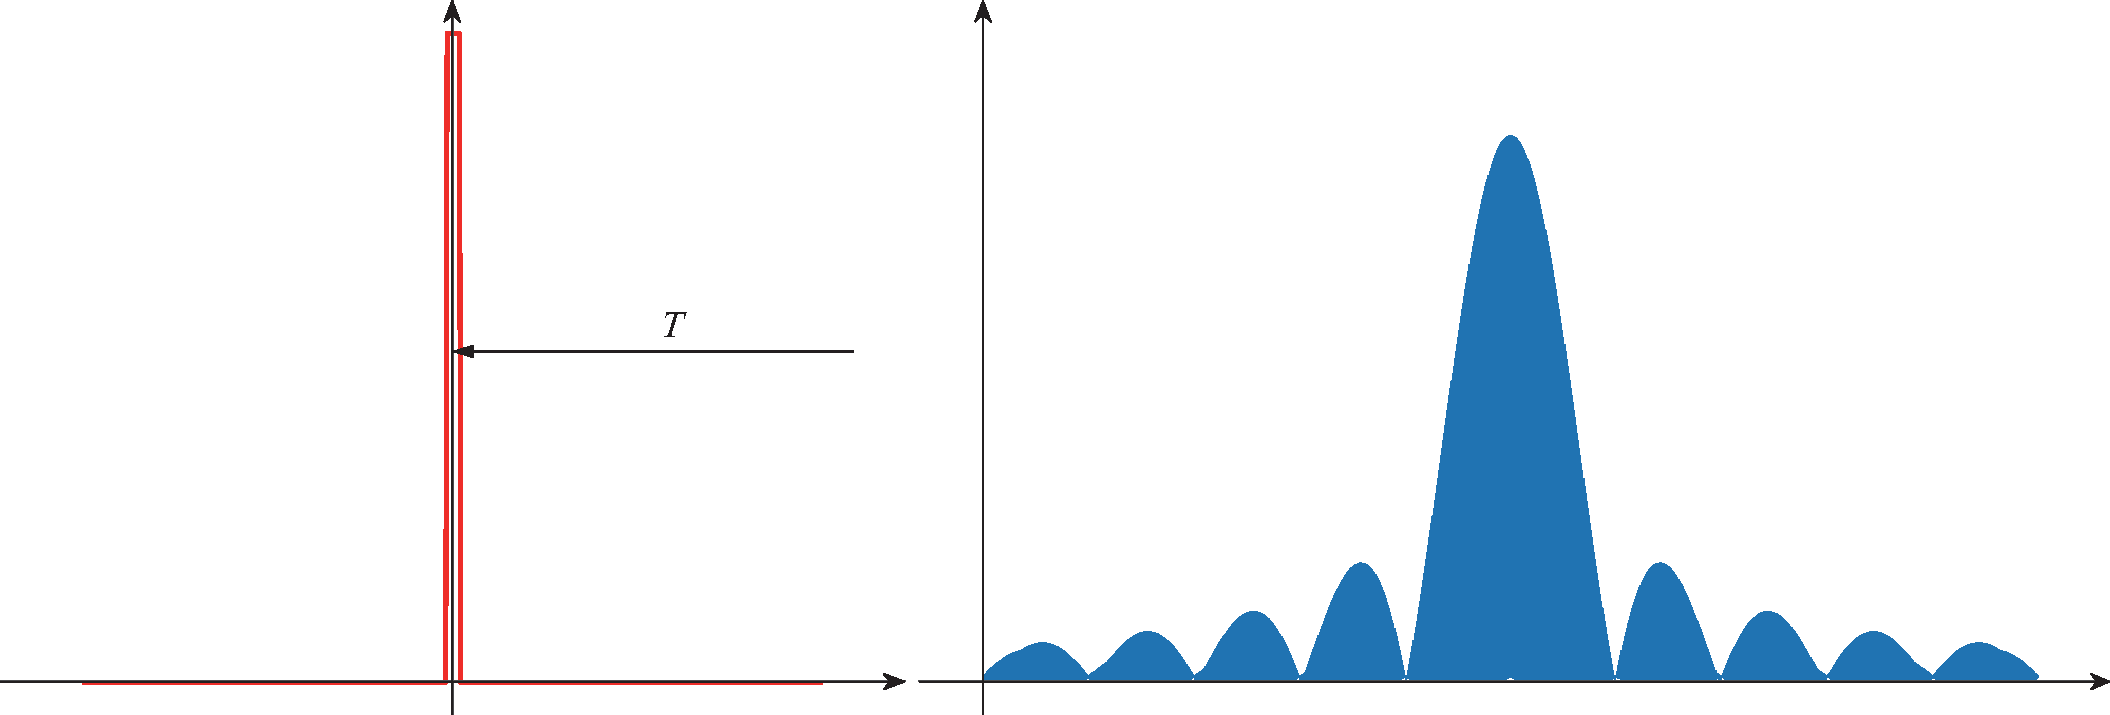
\includegraphics[width=0.5\linewidth]{pic/Fo3.pdf}};
		\node (E) [draw, inner sep = 5pt, below of = D, node distance = 3.5cm]{\makecell[c]{正弦函数又对应圆周运动的投影,\\而$\e^{\i \omega x}$恰好表示频率为$\omega$的单位圆周运动}};
		\node (F) [draw, inner sep = 5pt, right of = E, node distance = 9cm]{\makecell[c]{正弦函数的叠加 $\, \rightarrow \,$ 圆周运动的叠加 $\, \rightarrow \, $ $\e^{\i \omega x}$ 的叠加}};
		\node (G) [draw, inner sep = 5pt, below of = E, node distance = 3.5cm, xshift = 5cm]{$\displaystyle f(x) \sim \mathop{\underbrace{\int_{- \infty}^{+ \infty} \quad \mathop{F(\omega)}_{\makecell[c]{\\[-2em] \scriptsize \mbox{圆周运动的半径}\\[-0.7em] \scriptsize \mbox{和相位信息}\\[-0.7em]}} \quad \mathop{\e^{\i \omega x}}_{\makecell[c]{\scriptsize \mbox{以} {\scriptstyle \omega} \mbox{为频率绕原点}\\[-0.7em] \scriptsize \mbox{做圆周运动的向量}\\[-0.7em]}} \quad \d \omega}}_{\scriptsize \mbox{叠加}}$};
		
		\draw[arrows={-Stealth[scale=0.8]}] (A) -- (B);
		\draw[arrows={-Stealth[scale=0.8]}] (B) -- (C);
		\draw[arrows={-Stealth[scale=0.8]}] (C) -- (D);
		\draw[arrows={-Stealth[scale=0.8]}] (D) -- (E);
		\draw[arrows={-Stealth[scale=0.8]}] (E) --+ (0cm, -1.75cm) --+(5cm, -1.75cm) -- (G);
		\draw[arrows={-Stealth[scale=0.8]}] (F) --+ (0cm, -1.75cm) --+(-4cm, -1.75cm) -- (G);
		\draw (B) -- (B1);
		\draw (C) -- (C1);
		\draw (D) -- (D1);
	\end{tikzpicture}
	\caption{Fourier变换的理解图}
	\label{Fourier变换的理解图}
\end{figure}


\subsection{Fourier变换的基本性质}
\begin{enumerate}[\textbf{性质} 1 ]
	\item \textbf{线性性质} 
	\begin{align}
		\mathcal{F}\big[C_1f_1 + C_2 f_2\big] = C_1 \mathcal{F}\big[f_1\big] + C_2 \mathcal{F}\big[f_2\big] 
	\end{align}
	
	\item \textbf{微分性质}
	\begin{align}
		\mathcal{F}\big[f'(x)\big] &= \i \omega \mathcal{F}\big[f(x)\big]\\[0.5em]
		\mathcal{F}\big[f^{(m)}(x)\big] &= (\i \omega)^{m} \mathcal{F}\big[f(x)\big]
	\end{align}
	
	\item \textbf{象函数微分性质}
	\begin{align}
		\mathcal{F}\big[xf(x)\big] &= \i \dfrac{\d }{\d \omega}\mathcal{F}\big[f(x)\big]\\[0.5em]
		\mathcal{F} \big[x^m f(x)\big] &= \i^m \dfrac{\d^m}{\d \omega^m} \mathcal{F}\big[f(x)\big]
	\end{align}
	
	\item \textbf{卷积性质}
	\begin{itemize}
		\item 卷积定义
		\begin{align}
			f_1(x) * f_2(x) = \int_{- \infty}^{+ \infty} f_1(t)f_2(x - t)\, \d t
		\end{align}
		\item 卷积性质
		\begin{align}
			\mathcal{F}\big[f_1(x) * f_2(x)\big] &= \mathcal{F}\big[f_1(x)\big] \cdot \mathcal{F}\big[f_2(x)\big]\\[0.5em]
			f_1(x) * f_2(x) &= \mathcal{F}^{-1}\big[F_1(\omega)\cdot F_2(\omega)\big]
		\end{align}
	\end{itemize}
\end{enumerate}

\subsection{{$\delta$}函数及其Fourier变换}
\begin{enumerate}[1. ]
	\item $\delta$函数的定义
	\begin{enumerate}[\textbf{特征} 1 ]
		\item \textbf{无穷高且窄}
		\begin{align}
			\delta (x - x_0) = \,
			\begin{cases}
				0, & x \neq x_0\\
				\infty, & x = 0
			\end{cases}
		\end{align}
		
		\item \textbf{具有单位面积}\quad $\displaystyle \int_{- \infty}^{+ \infty} \delta(x - x_0)\, \d x = 1$
	\end{enumerate}
	
	\item $\delta$ 函数的性质
	\begin{enumerate}[\textbf{性质} 1 ]
		\item \textbf{筛选性质} \quad $\displaystyle \int_{- \infty}^{+ \infty} f(x)\delta(x - x_0) \, \d x = f(x_0)$
		\item \textbf{偶函数} \quad $\delta(x) = \delta(-x)$
		\item \textbf{卷积表平移} \quad $\displaystyle \delta(x - a)*f(x) = \int_{- \infty}^{+ \infty} \delta(\xi - a)f(x - \xi) \, \d \xi = f(x - a)$ 
	\end{enumerate}
	
	\item $\delta$函数的Fourier变换
	\begin{align}
		\mathcal{F}\big[\delta(x - x_0)\big] = \int_{-\infty}^{\infty} \delta(x - x_0) \e^{-\i \omega x}\, \d x = 1
	\end{align}
\end{enumerate}
\clearpage

\section{Laplace变换}
\vspace*{1em}
\ttheorem[Laplace变换]
\dy[Laplace变换]{LaplaceBH}
\begin{align}
	F(p) = \mathcal{L}\big[f(t)\big] = \int_{0}^{+ \infty} f(x) \e^{- p t}\, \d x
\end{align}
\vspace*{-2em}

\dy[反演]{FY}
\begin{align}
	f(t) = \mathcal{L}^{-1} \big[F(p)\big] = \dfrac{1}{2 \pi \i} \int_{\beta - \i \infty}^{\beta + \i \infty} F(p) \e^{pt}\, \d p
\end{align}

\subsection{Laplace变换的理解}
\begin{figure}[!htb]
	\centering
	\begin{tikzpicture}
		\node (A) [draw, inner sep = 5pt]{\makecell[c]{我们想求函数$g(t)$的 Fourier变换,然而\\当$t\to \infty, g(t) \to \infty$,不满足绝对可积}};
		\node (AB) [draw, inner sep = 3pt, right of = A, node distance = 7.2cm, yshift = - 2cm]{\makecell[c]{不关心$t<0$时的情况}};
		\node (B) [draw, inner sep = 5pt, below of = A, node distance = 3.5cm]{\makecell[c]{构造新函数}};
		\node (BC) [draw, inner sep = 3pt, right of = B, node distance = 7.5cm, yshift = - 1.75cm]{\makecell[l]{乘以一个衰减函数$\e^{- \beta t}$\\乘以一个单位阶跃函数$u(t)$}};
		\node (C) [draw, inner sep = 7pt, below of = B, node distance = 4cm,]{$g(t) \hspace*{0.5em} \cdot \hspace*{0.5em} \mathop{u(t)}\limits_{\makecell[c]{\\[-2em]\scriptsize \mbox{单位阶跃函数,使}\\[-0.7em] \scriptsize \scriptstyle t < 0\mbox{,函数值为0}\\[-0.7em]}} \hspace*{0.5em} \cdot \hspace*{0.5em} \mathop{\e^{-\beta t}}\limits_{\makecell[c]{\scriptsize \mbox{衰减函数,使}\\[-0.7em] \scriptsize \scriptstyle g(t)\mbox{绝对可积}\\[-0.7em]}}  $};
		\node (CD) [draw, inner sep = 3pt, right of = C, node distance = 7.2cm, yshift = - 2cm]{\makecell[c]{对新函数作Fourier变换}};
		\node (D) [draw, inner sep = 5pt, below of = C, node distance = 3.5cm]{$\displaystyle F(\beta + \i \omega) = \int_{- \infty}^{+ \infty}g(t)u(t)\e^{- \beta t} \e ^{- \i \omega t} \, \d t$};
		\node (DE) [draw, inner sep = 2pt, right of = D, node distance = 6.4cm, yshift = - 2.2cm]{\makecell[l]{$f(t) = g(t) u(t)$ \\ $p = \beta + \i \omega $}};
		\node (E) [draw, inner sep = 5pt, below of = D, node distance = 4cm]{$\displaystyle F(p) = \int_{0}^{+ \infty}f(t) \e ^{- p t} \, \d t$};
		
		\draw[arrows={-Stealth[scale=0.8]}] (A) -- (B);
		\draw[arrows={-Stealth[scale=0.8]}] (B) -- (C);
		\draw[arrows={-Stealth[scale=0.8]}] (C) -- (D);
		\draw[arrows={-Stealth[scale=0.8]}] (D) -- (E);
		\draw[arrows={-Stealth[scale=0.8]}] (AB) -- +(-7.2cm, 0cm);
		\draw[arrows={-Stealth[scale=0.8]}] (BC) -- +(-7.5cm, 0cm);
		\draw[arrows={-Stealth[scale=0.8]}] (CD) -- +(-7.2cm, 0cm);
		\draw[arrows={-Stealth[scale=0.8]}] (DE) -- +(-6.4cm, 0cm);
	\end{tikzpicture}
	\caption{Laplace变换的理解图}
	\label{Laplace变换的理解图}
\end{figure}


\subsection{Laplace变换的性质}

\begin{enumerate}[\textbf{性质} 1 ]
	\item \textbf{线性性质}\\
	若$\alpha,\beta$是任意常实数,且$\mathcal{L}\big[f_1(t)\big] = F_1(s), \mathcal{L}\big[f_2(t)\big] = F_2(s)$,则有
	\begin{equation}
		\mathcal{L}\big[\alpha f_1(t)\pm \beta f_2(t)\big] = \alpha F_1(s) \pm \beta F_2(s)
	\end{equation}
	
	\item \textbf{微分性质}\\
	若$\mathcal{L}\big[f(t)\big] = F(s)$,则有
	\begin{equation}
		\mathcal{L}\big[f^{(n)}(t)\big] = s^nF(s) -s^{n-1}f(0)-s^{n-2}f'(0)- \cdots - f^{(n-1)}(0)
	\end{equation}
	
	\item \textbf{积分性质}\\
	若$\mathcal{L}\big[f(t)\big] = F(s)$,则有
	\begin{equation}
		\mathcal{L}\left[\underbrace{\int\cdots\int}_{n} f(t) \,\d t^n\right]=\frac{1}{s^n}F(s)+\frac{1}{s^n}f^{-1}(0) +\frac{1}{s^{n-1}}f^{(-2)}(0)+\cdots +\frac{1}{s}f^{(-n)}(0)
	\end{equation}
	其中,$f^{(-1)}(0),f^{(-2)}(0),f^{(-n)}(0)$分别为$f(t)$的各重积分在$t=0$处的值。\\
	
	\item \textbf{卷积定理}\\
	若$\mathcal{L}\big[f_1(t)\big] = F_1(s), \mathcal{L}\big[f_2(t)\big] = F_2(s)$,则
	\begin{equation}
		\mathcal{L}\big[f_1(t) * f_2(t)\big] = F_1(s) \cdot F_2(s)
	\end{equation}
\end{enumerate}
\warn[
Laplace变换的重要条件:\vspace*{-0.5em}
{
	\begin{enumerate}
		\item $t<0$时,$f(t)=0$;$t > 0$时,$f(t)$是分段光滑的。\vspace*{-0.5em}
		\item $f(t)$有\textcolor{red}{有限的增长指数}。即存在正数$M$及$c \ge 0$,使得对于任何$t$值,$|f(t)| \le M\e^{ct}$,则Laplace变换在$\text{Re} (p)= \beta >c$时存在。
	\end{enumerate}
}
]

\subsection{Laplace反演的计算}
\noindent \textbf{1. 留数定理}
\begin{enumerate}[\hspace*{2em}(1) ]
	\item 极点的判断方法:\textbf{$\dfrac{1}{f(p)}$的$m$重零点就是$f(p)$的$m$级极点}.
	\item $n$级极点的留数:设$p_0$是函数$f(p)$的$n$级极点,则
	\begin{equation}
		\text{Res} [f(p), p_0] = \dfrac{1}{(n-1)!} \lim\limits_{p \to p_0} \dfrac{\d^{n-1}\big[(p - p_0)^n f(p)\big]}{\d p^{n-1}}
	\end{equation}
\end{enumerate}


\noindent \textbf{2. 反演公式转换为求极点留数}

设$p_1,p_2,\cdots,p_n$是函数$F(p)$的所有奇点,适当选取$\Re (p) = \beta$使这些奇点落在复平面上直线$\Re(p) = \beta$的左侧,且$\bm{p \to \infty,  F(p) \to 0}$,则
\begin{align}
	f(t) = \sum_{k = 0}^n \text{Res}\big[F(p)\e^{pt}, p_k\big]
\end{align}

\subsection{Laplace变换的应用——求解常微分方程(组)}
\texample[Laplace变换求解常微分方程(组)]\vspace*{2em}
\noindent \vspace*{1.5em} \noindent  \hspace*{0.2em}  \tcbox[colframe =black, colback =black!10!white,boxrule=0.5mm,size=small,on line]{\color{black}{{ 解题步骤}}\hspace*{0.25em}}\hspace{1.5em}
\vspace*{-1em}
\begin{enumerate}
	\item 对方程两边同时做拉普拉斯变换。
	\item 利用拉普拉斯变换的线性性质、微分性质代替各阶的的导数,解出$Y(s)$。
	\item 做$Y(s)$的拉普拉斯逆变换,得到$y(t)$。
\end{enumerate}
\warn[
\textbf{Fourier变换和Laplace变换的对比}\vspace*{-0.5em}
{
	\begin{enumerate}
		\item 都属于积分变换,实函数变换为复函数,但积分范围不同。\vspace*{-0.5em}
		\item 存在条件\vspace*{-0.5em}
		\begin{itemize}
			\item Fourier \quad 分段光滑,绝对可积
			\item Laplace \quad 分段光滑,$f(t)$增长小于指数级
		\end{itemize}
		\item 积分变量不同\vspace*{-0.5em}
		\begin{itemize}
			\item Fourier \quad $\omega \in (- \infty , + \infty)$
			\item Laplace \quad $p$的实部满足一定条件(可自行调节)
		\end{itemize}
	\end{enumerate}
}
]

\section{积分变换法}
\subsection{积分变换法简述}
\noindent \textbf{1. 积分变换的性质}
\begin{enumerate}[\hspace*{1em}\textbf{性质} 1 ]
	\item \textbf{积分变换的微分性质}
	\begin{align}
		\mathcal{F}\big[f'(x)\big] &=  \i \omega \mathcal{F}\big[f(x)\big] \\[0.5em]
		\mathcal{F}\big[f''(x)\big] &=  -\omega^2 \mathcal{F}\big[f(x)\big] \\[1em]
		\mathcal{L}\big[f'(t)\big] & = p \mathcal{L}\big[f(t)\big] - f(0)\\[0.5em]
		\mathcal{L}\big[f''(t)\big] & = p^2\mathcal{L}\big[f(t)\big] - pf(0) - f'(0)
	\end{align}
	
	\item \textbf{积分变换的卷积性质}
	\begin{align}
		f_1(x) * f_2(x) &= \int_{-\infty}^{+\infty} f_1(\xi)f_2(x - \xi) \, \d \xi  = \mathcal{F}^{-1}\big[F_1(\omega)\cdot F_2(\omega)\big]\\[1em]
		f_1(t) * f_2(t) &= \int_{0}^{t} f_1(\tau)f_2(t - \tau) \, \d \tau = \mathcal{L}^{-1}\big[F_1(p)\cdot F_2(p)\big]
	\end{align}
\end{enumerate}

\noindent \textbf{2. 积分变换法的基本步骤}
\begin{enumerate}[\hspace*{1em}\textbf{步骤} 1 ]
	\item \textbf{变换} \quad 选适当的积分变换,对方程的两边做变换将偏微分方程变为含参量的常微分方程;对变换中未利用到的定解条件也做变换。关于积分变量的选取,与两个变换方法的积分域有关:
	\begin{itemize}
		\item Fourier变换 \quad 积分域为$(-\infty, + \infty) \quad \Rightarrow \quad$无界空间变量
		\item Laplace变换 \quad 积分域为$(0, +\infty) \quad \Rightarrow \quad$时间变量
		\item 如果同时存在无界空间变量和时间变量,这时可以联用两种变换,即\dy[联合变换]{LHBH}
	\end{itemize}
	\item \textbf{求解} \quad 解常微分方程,得到像函数的解
	\begin{itemize}
		\item 一阶齐次方程 \quad 分离变量法
		\item 二阶齐次方程\quad 特征根法
		\item 非齐次方程\quad 常数变易法
	\end{itemize}
	\item \textbf{反演} \quad 对像函数反演,得到原定解问题的解,通常有以下两个解法
	\begin{itemize}
		\item 查表$+$卷积性质
		\item 留数定理
	\end{itemize}
\end{enumerate}
\vspace*{-1em}

\warn[
\begin{itemize}
	\item 在用积分变换求解定解问题时,假定所求的解及定解条件 中的已知函数的变换都是存在的;\vspace*{-0.5em}
	\item 一个未知函数在未求出前是很难判断变换是否存在的,因此,在未做验证前,得到的只是形式解。
\end{itemize}
]

\subsection{积分变换法举例}
\begin{equation*}
	\mbox{积分变换法} \, 
	\begin{cases}
		\, \mbox{热传导方程} \,
		\begin{cases}
			\, \mbox{无界杆的热传导问题}\\
			\, \mbox{半无界杆的热传导问题}\\
		\end{cases}
		\\
		\, \mbox{波动方程} \,
		\begin{cases}
			\, \mbox{无界弦的自由振动}\\
			\, \mbox{无界弦的受迫振动}\\
			\, \mbox{有界杆的受迫振动}
		\end{cases}
	\end{cases}
\end{equation*}
\vspace*{1em}

\example[无界杆上的热传导问题]
设有一个根无限长的杆,杆上具有强度为$F(x,t)$的热源,杆的初始温度为$\varphi(x)$,试求$t>0$时杆上温度的分布规律。

\solve 方法一:Fourier变换
\begin{enumerate}[\textbf{第} 1 \textbf{步} ]
	\item \textbf{列出定解问题}
	\begin{equation}
		\begin{cases}
			\, \dfrac{\partial u}{\partial t} = a^2 \dfrac{\partial^2 u}{\partial x^2} + f(x,t), & -\infty < x< +\infty,t>0\\[0.5em]
			\, u|_{t = 0} = \varphi(x), & -\infty < x < + \infty
		\end{cases}
	\end{equation}
	其中,$\displaystyle a^2 \dfrac{\lambda}{\rho c}$表示热扩散系数,$f(x,t) = \dfrac{F(x,t)}{\rho c}$.可以分析得到:
	\begin{itemize}
		\item 具有无界空间变量$x$,可进行Fourier变换;
		\item 具有时间变量$t$,可进行Laplace变换;
		\item 可以单独采用一种变换,也可以两种联用;
	\end{itemize}
	
	\item \textbf{变换}
	\begin{itemize}
		\item 取$x$为变换变量,对方程和定解条件进行Fourier变换
		\begin{equation}
			\begin{cases}
				\, \dfrac{\displaystyle \partial \int_{-\infty}^{+\infty} u(x,t)\e^{- \i \omega x} \, \d x}{\partial t} = \displaystyle a^2 \int_{- \infty}^{+ \infty} \dfrac{\partial^2 u(x,t)}{\partial x^2} \e^{- \i \omega x}\, \d x + \int_{- \infty}^{+\infty}\e^{- \i \omega x} \, \d x\\[1em]
				\, \displaystyle \int_{-\infty}^{+\infty} u(x,0) \e^{- \i \omega x}\, \d x = \int_{- \infty}^{+ \infty}\varphi(x)\e^{-\i \omega x} \, \d x
			\end{cases}
		\end{equation}
		
		\item 记$U = \mathcal{F}[u], G = \mathcal{F}[f], \varPhi = \mathcal{F}[\varphi]$,则
		\begin{equation}
			\begin{cases}
				\, \dfrac{\d U(\omega, t)}{\d t} = - a^2 \omega^2U(\omega, t) + G(\omega, t)\\
				\, U(\omega, t)|_{t = 0} = \varPhi(\omega)
			\end{cases}
		\label{无界杆传热}
		\end{equation}
	\end{itemize}
	
	\item \textbf{求解}\\
	方程\eqref{无界杆传热}是以$\omega$为参变量的一阶线性非齐次常微分方程,利用常数变易法解得
	\begin{equation}
		U(\omega, t) = \varPhi(\omega)\exp\left(-a^2 \omega^2 t\right) + \int_0^t G(\omega ,\tau) \exp \big[-a^2 \omega^2(t - \tau)\big]\, \d \tau
	\end{equation}
	
	\item \textbf{反演}
	\begin{itemize}
		\item 查表可得
		\[
		\begin{cases}
			\, \mathcal{F}^{-1}\left[\exp\left(-a^2 \omega^2 t\right)\right] = \dfrac{1}{2a\sqrt{\pi t}}\exp \left(-\dfrac{x^2}{4a^2t}\right)\\[1em]
			\, \mathcal{F}^{-1}\bigg\lbrace\exp\left[-a^2 \omega^2 (t-\tau)\right]\bigg\rbrace = \dfrac{1}{2a\sqrt{\pi (t-\tau)}}\exp \left(-\dfrac{x^2}{4a^2(t - \tau)}\right)
		\end{cases}
		\]
		
		\item 卷积性质
		\begin{align}
			u(x,t) &= \varphi(x) * \Bigg[\dfrac{1}{2 a \sqrt{\pi t}}\exp\left(-\dfrac{x^2}{4a^2t}\right)\Bigg]\notag \\[1em]
			&\quad +\int_{0}^{t} \Bigg\lbrace f(x, \tau) * \dfrac{1}{2a\sqrt{\pi (t - \tau)}}\exp \left[-\dfrac{x^2}{4a^2(t - \tau)}\right] \Bigg \rbrace \, \d \tau \notag \\[1em]
			& = \dfrac{1}{2a\sqrt{\pi t}}\int_{-\infty}^{+\infty}\varphi(\xi)\exp\left[-\dfrac{(x - \xi)^2}{4a^2t}\right]\, \d \xi \notag\\[1em]
			&\quad + \dfrac{1}{2a \sqrt{\pi}} \int_0^t\int_{-\infty}^{+\infty}\dfrac{f(\xi, \tau)}{\sqrt{t - \tau}} \exp \left[-\dfrac{(x - \xi)^2}{4a^2(t - \tau)}\right]\, \d \xi \d \tau
		\end{align}
	\end{itemize}
\end{enumerate}

	\solveother 方法二:联合变换求解
\begin{enumerate}[\textbf{第} 1 \textbf{步} ]
	\item \textbf{列出定解问题}
	\begin{equation}
		\begin{cases}
			\, \dfrac{\partial u}{\partial t} = a^2 \dfrac{\partial^2 u}{\partial x^2} + f(x,t), & -\infty < x< +\infty,t>0\\[0.5em]
			\, u|_{t = 0} = \varphi(x), & -\infty < x < + \infty
		\end{cases}
	\end{equation}
	\item \textbf{变换}
		\begin{itemize}
			\item 取$x$为变换变量,对方程和定解条件进行Fourier变换,记$U = \mathcal{F}[u], G = \mathcal{F}[f], \varPhi = \mathcal{F}[\varphi]$,则
			\begin{equation}
				\begin{cases}
					\, \dfrac{\d U(\omega, t)}{\d t} = - a^2 \omega^2U(\omega, t) + G(\omega, t)\\
					\, U(\omega, t)|_{t = 0} = \varPhi(\omega)
				\end{cases}
			\end{equation}
			\item 再对变量$t$作Laplace变换:
			\begin{equation}
				\int_{0}^{\infty} \dfrac{\d U(\omega, t)}{\d t} \e^{- p t} \, \d t = -a^2\omega^2\int_{0}^{\infty} U(\omega, t)\e^{-p t} \, \d t + \int_{0}^{\infty}G(\omega, t)\e^{-pt}\, \d t
			\end{equation}
		\end{itemize}	
	引入$\sim$符号表示像函数,得到代数方程
	\begin{equation}
		p \widetilde{U}(\omega , p) - \varPhi(\omega) = -a^2 \omega^2 \widetilde{U}(\omega, p) + \widetilde{G}(\omega, p)
		\label{无界杆传热2}
	\end{equation}
	
	\item \textbf{求解}\\
	方程\eqref{无界杆传热2}是线性方程,直接解得
	\begin{equation}
		\widetilde{U}(\omega, p) = \dfrac{1}{p + a^2 \omega^2}\varPhi(\omega) + \dfrac{1}{p + a^2 \omega^2} \widetilde{G}(\omega, p)
	\end{equation}
	
	\item \textbf{反演}\\
	(1) 先对变量$p$进行反演
	\begin{itemize}
		\item 查表可得
		\[
		\mathcal{L}^{-1}\left[\dfrac{1}{p + a^2 \omega^2}\right] = \exp\left(-a^2 \omega^2 t\right)
		\]
		
		\item 卷积性质
		\begin{align}
			U(\omega, p) &= \mathcal{L}^{-1}\left[\dfrac{1}{p + a^2 \omega^2}\varPhi(\omega) + \dfrac{1}{p + a^2 \omega^2} \widetilde{G}(\omega, p)\right] \notag\\
			& = \varPhi(\omega) \exp\left(-a^2 \omega^2 t\right) + G(\omega, t)*\exp\left(-a^2 \omega^2 t\right) \notag\\
			& = \varPhi(\omega) \exp\left(-a^2 \omega^2 t\right) + \int_0^t G(\omega, t)*\exp\left[-a^2 \omega^2 (t - \tau)\right]\, \d \tau
		\end{align}
	\end{itemize}
	(2) 再对变量$\omega$进行反演,此步骤与方法一完全相同,略。
\end{enumerate}
\vspace*{4em}

\example[半无界杆上的热传导问题]
设有一根半无限长的杆,端点温度变化为已知,杆的初始温度为$0\degree \text{C}$,求杆上的温度分布规律。

\solve 利用Laplace变换求解
\begin{enumerate}[\textbf{第} 1 \textbf{步} ]
	\item \textbf{列出定解问题}
	\begin{equation}
		\begin{cases}
			\, \dfrac{\partial u}{\partial t} = a^2 \dfrac{\partial^2 u}{\partial x^2}, & x>0,t>0\\
			\, u|_{x = 0} = f(t), & t > 0\\
			\, u|_{t = 0} = 0, & x > 0
		\end{cases}
	\end{equation}
	\clearpage
	可以分析得到:
	\begin{itemize}
		\item 没有无界空间变量$x$,不可以进行Fourier变换;
		\item 具有时间变量$t$,可进行Laplace变换。
	\end{itemize}
	
	\item \textbf{变换}
	\begin{itemize}
		\item 取$t$为变换变量,对方程和定解条件进行Laplace变换
		\begin{equation}
			\begin{cases}
				\, \dfrac{\displaystyle \partial \int_{0}^{+\infty} u(x,t)\e^{- p t} \, \d t}{\partial t} = \displaystyle a^2 \int_{0}^{+ \infty} \dfrac{\partial^2 u(x,t)}{\partial x^2} \e^{- p t}\, \d t \\[1em]
				\, \displaystyle \int_{0}^{+\infty} u(0,t) \e^{- p t}\, \d t = \int_{0}^{+ \infty}f(t)\e^{-pt} \, \d t
			\end{cases}
		\end{equation}
		
		\item 记$U = \mathcal{L}[u],F = \mathcal{L}[f]$,则
		\begin{equation}
			\begin{cases}
				\, \dfrac{\d^2 U(x, p)}{\d x^2} - \dfrac{p}{a^2} U(\omega, t) = 0 \\
				\, U(x, p)|_{x = 0} = F(p)
			\end{cases}
			\label{半无界杆传热}
		\end{equation}
	\end{itemize}
	
	\item \textbf{求解}\\
	方程\eqref{半无界杆传热}是以$p$为参变量的一阶线性齐次常微分方程,利用特征根法得其通解为
	\begin{equation}
		U(x, p) = C_1 \exp \left(\dfrac{\sqrt{p}}{a}x\right) + C_2\exp \left(-\dfrac{\sqrt{p}}{a}x\right) 
	\end{equation}
	由于$x \to \infty, U \to C$(常数),所以为了保证$U(x, p)$的有界性,无穷发散量$\exp \left(\dfrac{\sqrt{p}}{a}x\right)$的系数$C_1 = 0.$
	
	再根据边界条件得到方程的特解
	\begin{equation}
		U(x, p) = F(p) \exp\left(-\dfrac{p}{a^2}x\right)
	\end{equation}
	
	\item \textbf{反演}
	\begin{itemize}
		\item 查表可得
		\[
		\mathcal{L}\Bigg[\text{erfc}\left(\dfrac{x}{2a\sqrt{t}}\right)\Bigg] = \dfrac{1}{p}\exp \left(-\dfrac{\sqrt{p}}{a}\right)
		\]
		
		\item 微分性质
		\[
		\mathcal{L} \Bigg[\dfrac{\d }{\d t}\text{erfc}\left(\dfrac{x}{2a\sqrt{t}}\right)\Bigg] = p \mathcal{L}\Bigg[\text{erfc}\left(\dfrac{x}{2a\sqrt{t}}\right)\Bigg] - \text{erfc}(\infty) = p \cdot \dfrac{1}{p}\exp \left(-\dfrac{\sqrt{p}}{a}\right) - 0 = \exp \left(-\dfrac{\sqrt{p}}{a}\right) 
		\]
		所以
		\begin{equation}
			\mathcal{L}^{-1}  \Bigg[\exp \left(-\dfrac{\sqrt{p}}{a}\right)  \Bigg] = \dfrac{\d }{\d t}\text{erfc}\left(\dfrac{x}{2a\sqrt{t}}\right) = \dfrac{x}{2a \sqrt{\pi} t^{3/2}}\exp \left(-\dfrac{x^2}{4a^2t}\right)
		\end{equation}
		
		\item 卷积性质
		\begin{equation}
			u(x, t) = \mathcal{L}^{-1}\big[U(x, p)\big] = \dfrac{x}{2a \sqrt{\pi}}\int_0^t \dfrac{f(\tau)}{(t - \tau)^{3/2}} \exp \left[- \dfrac{x^2}{4a^2(t - \tau)}\right]\, \d \tau
		\end{equation}
	\end{itemize}
\end{enumerate}
\clearpage

\example[无界弦的自由振动]
试分析无界弦的自由振动。

\solve 利用Fourier变换求解
\begin{enumerate}[\textbf{第} 1 \textbf{步} ]
	\item \textbf{列出定解问题}
	\begin{equation}
		\begin{cases}
			\, \dfrac{\partial^2 u}{\partial t^2} = a^2 \dfrac{\partial^2 u}{\partial x^2} , & -\infty < x< +\infty,t>0\\[0.5em]
			\, u|_{t = 0} = \varphi(x), & -\infty < x < + \infty\\[0.5em]
			\,\left. \dfrac{\partial u}{\partial t}\right|_{t = 0} = \psi(x), & -\infty < x < +\infty
		\end{cases}
	\end{equation}
	可以分析得到:
	\begin{itemize}
		\item 具有无界空间变量$x$,可进行Fourier变换;
		\item 具有时间变量$t$,可进行Laplace变换;
		\item 可以单独采用一种变换,也可以两种联用;
	\end{itemize}
	
	\item \textbf{变换}
	\begin{itemize}
		\item 取$x$为变换变量,对方程和定解条件进行Fourier变换
		\begin{equation}
			\begin{cases}
				\, \displaystyle \dfrac{\partial^2}{\partial t^2} \int_{-\infty}^{+\infty} u(x,t)\e^{- \i \omega t} = a^2 \int_{- \infty}^{+\infty} \dfrac{\partial^2 u(x,t)}{\partial x^2} \e^{- \i \omega x}\,\d x \\[1em]
				\, \displaystyle \left[\int_{- \infty}^{+\infty}u(x,t)\e^{-\i \omega x}\, \d x\right]_{t = 0} = \int_{-\infty}^{+ \infty} \varphi(x)\, \d x \\[1em]
				\, \displaystyle \left[\int_{- \infty}^{+\infty} \dfrac{\partial u(x,t)}{\partial t}\e^{- \i \omega x}\, \d x\right]_{t = 0} = \int_{- \infty}^{+\infty} \psi(x)\e^{- \i \omega x} \, \d x
			\end{cases}
		\end{equation}
		
		\item 记$U = \mathcal{F}[u], \varPhi = \mathcal{F}[\varphi], \varPsi = \mathcal{F}[\psi]$,则
		\begin{equation}
			\begin{cases}
				\, \displaystyle \dfrac{\d^2 U(\omega, t)}{\d t^2} = -a^2 \omega^2 U(\omega, t)\\[0.5em]
				\, \displaystyle U(\omega, t)|_{t = 0} = \varPhi(\omega)\\[0.5em]
				\, \displaystyle \left. \dfrac{\d U(\omega, t)}{\d t} \right|_{t = 0} = \varPsi(\omega)
			\end{cases}
			\label{无界弦自由振动}
		\end{equation}
	\end{itemize}
	
	\item \textbf{求解}\\
	方程\eqref{无界弦自由振动}是以$\omega$为参变量的二阶线性齐次常微分方程,利用特征根法解得
	\begin{itemize}
		\item 通解
		\begin{equation}
			U(\omega, t) = A\cos a\omega t + B\sin a \omega t
		\end{equation}
		\item 特解
		\begin{equation}
			U(\omega, t) = \varPhi(\omega)\cos a\omega t + \varPsi(\omega) \dfrac{\sin a\omega t}{a \omega}
		\end{equation}
	\end{itemize}
	
	\item \textbf{反演}
	\begin{itemize}
		\item 利用欧拉公式变形
		\begin{align*}
			U(\omega, t) & = \varPhi(\omega)\cos a\omega t + \Psi(\omega)\dfrac{\sin a\omega t}{a \omega} \\
			& = \dfrac{1}{2}\big[\varPhi(\omega) \e^{\i a \omega t} + \varPhi(\omega)\e^{- \i a \omega t}\big] + \dfrac{1}{2a} \Bigg[\dfrac{1}{\i \omega}\varPsi(\omega) \e^{\i a \omega t} - \dfrac{1}{\i \omega} \varPsi(\omega) \e^{- \i a\omega t}\Bigg]
		\end{align*}
		\item 位移性质
		\begin{equation}
			f(x + x_0) = \mathcal{F}^{-1} \big[\e^{\i \omega x_0}F(\omega)\big]
		\end{equation}
		
		\item 积分性质
		\begin{equation}
			\int_{-\infty}^x f(\xi) \, \d \xi = \mathcal{F}^{-1} \Bigg[\dfrac{1}{\i \omega}F(\omega)\Bigg]
		\end{equation}
		
		\item 将位移性质作用于积分性质
		\begin{equation}
			\int_{-\infty}^{x + x_0} f(\xi)\, \d \xi = \mathcal{F}^{-1} \Bigg[\dfrac{1}{\i \omega} F(\omega) \e^{\i \omega x_0}\Bigg]
		\end{equation}
		
		所以
		\begin{align}
			u(x, t) &= \dfrac{1}{2} \big[\varphi(x + at) + \varphi(x - at)\big] + \dfrac{1}{2a}\Big[\int_{- \infty}^{x +at}\psi(\xi)\, \d \xi - \int_{-\infty}^{x - at} \psi(\xi) \, \d \xi\Big]\notag \\[1em]
			& = \dfrac{1}{2}\big[\varphi(x + at) + \varphi(x - at)\big] + \dfrac{1}{2a} \int_{x-at}^{x+at}\psi(\xi) \, \d \xi
		\end{align}
	\end{itemize}
\end{enumerate}

\example[无界弦的受迫振动]
试分析无界弦的受迫振动。

\solve 利用Fourier变换求解
\begin{enumerate}[\textbf{第} 1 \textbf{步} ]
	\item \textbf{列出定解问题}
	\begin{equation}
		\begin{cases}
			\, \dfrac{\partial^2 u}{\partial t^2} = a^2 \dfrac{\partial^2 u}{\partial x^2} + f(x,t), & -\infty < x< +\infty,t>0\\[0.5em]
			\, u|_{t = 0} = 0, & -\infty < x < + \infty\\[0.5em]
			\,\left. \dfrac{\partial u}{\partial t}\right|_{t = 0} = 0, & t-\infty < x < +\infty
		\end{cases}
	\end{equation}
	可以分析得到:
	\begin{itemize}
		\item 具有无界空间变量$x$,可进行Fourier变换;
		\item 具有时间变量$t$,可进行Laplace变换;
		\item 可以单独采用一种变换,也可以两种联用;
	\end{itemize}
	
	\item \textbf{变换}
	\begin{itemize}
		\item 取$x$为变换变量,对方程和定解条件进行Fourier变换
		\begin{equation}
			\begin{cases}
				\, \displaystyle \dfrac{\partial^2}{\partial t^2} \int_{-\infty}^{+\infty} u(x,t)\e^{- \i \omega t} = a^2 \int_{- \infty}^{+\infty} \dfrac{\partial^2 u(x,t)}{\partial x^2} \e^{- \i \omega x}\,\d x + \int_{- \infty}^{+\infty} f(x,t) \e^{- \i \omega x}\,\d x\\[1em]
				\, \displaystyle \left[\int_{- \infty}^{+\infty}u(x,t)\e^{-\i \omega x}\, \d x\right]_{t = 0} = 0\\[1em]
				\, \displaystyle \left[\int_{- \infty}^{+\infty} \dfrac{\partial u(x,t)}{\partial t}\e^{- \i \omega x}\, \d x\right]_{t = 0} = 0\,
			\end{cases}
		\end{equation}
		
		\item 记$U = \mathcal{F}[u], F= \mathcal{F}[f]$,则
		\begin{equation}
			\begin{cases}
				\, \displaystyle \dfrac{\d^2 U(\omega, t)}{\d t^2} = -a^2 \omega^2 U(\omega, t) + F(\omega, t)\\[0.5em]
				\, \displaystyle U(\omega, t)|_{t = 0} = 0\\[0.5em]
				\, \displaystyle \left. \dfrac{\d U(\omega, t)}{\d t} \right|_{t = 0} = 0
			\end{cases}
			\label{无界弦受迫振动}
		\end{equation}
	\end{itemize}
	
	\item \textbf{求解}\\
	方程\eqref{无界弦受迫振动}是以$\omega$为参变量的二阶线性非齐次常微分方程,利用常数变易法解得
		\begin{equation}
			U(\omega, t) = \dfrac{1}{a} \int_0^t F(\omega, t) \dfrac{\sin a\omega(t-\tau)}{\omega}\, \d \tau
		\end{equation}
	
	\item \textbf{反演}
	\begin{itemize}
		\item 查表,得
		\[
		\mathcal{F} \left[ f(x) =\, 
		\begin{cases}
			\, h, &- \tau < t < \tau\\
			\, 0, &\text{others}
		\end{cases}
		\right]
		 = 2h \dfrac{\sin \omega \tau}{\omega}
		\]
		经过变量替换,得到
		\[
		\dfrac{\sin a\omega(t - \tau)}{\omega} = \mathcal{F} \left[
		g(x) = \,
		\begin{cases}
			\, \dfrac{1}{2}, & -a(t - \tau) < x < a(t - \tau)\\
			\, 0, & \text{others}
		\end{cases}
		\right]
		\]
		\item 由卷积性质
		\begin{align}
			u(x, t) &= \dfrac{1}{2a} \int_0^t f(x,\tau) *g(x)\,\d \tau = \dfrac{1}{a} \int_0^t \int_{-\infty}^{+\infty} f(\xi, \tau) g(x - \xi) \, \d \xi \d \tau\\[0.5em]
			& = \dfrac{1}{2a} \int_{x-a(t - \tau)}^{x+a(t - \tau)}f(\xi, \tau) \, \d \xi
		\end{align}
	\end{itemize}
\end{enumerate}

\example[有界杆的受迫振动]
设有一根长为$l$的均匀杆,其一端固定,另一端由静止状态开始受力$F = A \sin \omega t$的作用,力$F$的方向与杆的轴线一致,求杆在零初值条件下作纵振动的规律。

\solve 利用Laplace变换求解
\begin{enumerate}[\textbf{第} 1 \textbf{步} ]
	\item \textbf{列出定解问题}
	\begin{equation}
		\begin{cases}
			\, \dfrac{\partial^2 u}{\partial t^2} = a^2 \dfrac{\partial^2 u}{\partial x^2} , & 0 < x< l,t>0\\[1em]
			\, u|_{t = 0} = 0, 	\,\left. \dfrac{\partial u}{\partial t}\right|_{t = 0} = 0, & 0 \le x \le l\\[1em]
			\, u|_{x = 0} = 0, 	\,\left. \dfrac{\partial u}{\partial t}\right|_{x = l} = \dfrac{A}{E}\sin \omega t, & t>0
		\end{cases}
	\end{equation}
	可以分析得到:
	\begin{itemize}
		\item 不具有无界空间变量$x$,不可进行Fourier变换;
		\item 具有时间变量$t$,可进行Laplace变换;
	\end{itemize}
	
	\item \textbf{变换}
	\begin{itemize}
		\item 取$t$为变换变量,对方程和定解条件进行Laplace变换
		\begin{equation}
			\begin{cases}
				\, \displaystyle \int_0^{+\infty} \dfrac{\partial^2 u(x,t)}{\partial t^2}\e^{-p t}\, \d t = a^2 \dfrac{\partial^2 }{\partial x^2} \int_0^{+\infty} u(x,t)\e^{- p t}\, \d t,\\[1em]
				\, \displaystyle \int_0^{+\infty} u(0,t) \e^{-pt}\, \d t = 0,\\[1em]
				\, \displaystyle \dfrac{\partial }{\partial x}\int_0^{+\infty} u(l,t)\e^{-pt}\, \d t = \dfrac{A}{E} \sin \omega t 
			\end{cases}
		\end{equation}
		
		\item 记$U = \mathcal{L}[u]$ 则
		\begin{equation}
			\begin{cases}
				\, \displaystyle p^2  U(x, p) = a^2 \dfrac{\d^2 U(x,p)}{\d x^2}\\[0.5em]
				\, \displaystyle U(x,p)|_{x = 0} = 0\\[0.7em]
				\, \displaystyle \left. \dfrac{\d U(x, p)}{\d x} \right|_{x = l} = \dfrac{A}{E} \dfrac{\omega}{p^2 + \omega^2}
			\end{cases}
			\label{有界弦受迫振动}
		\end{equation}
	\end{itemize}
	
	\item \textbf{求解}\\
	方程\eqref{有界弦受迫振动}是以$\omega$为参变量的二阶线性齐次常微分方程,利用特征根法解得
	\begin{itemize}
		\item 通解
		\begin{equation}
			U(x,p) = C_1 \exp\Bigg(\dfrac{p}{a} x\Bigg) +  C_2 \exp\Bigg(-\dfrac{p}{a} x\Bigg) 
		\end{equation}
		\item 特解
		\begin{align}
			U(x, p) = \dfrac{Aa\omega}{Ep(p^2 + \omega^2)} \dfrac{\exp\Bigg(\dfrac{p}{a} x\Bigg) - \exp\Bigg(-\dfrac{p}{a} x\Bigg)}{\exp\Bigg(\dfrac{p}{a} l\Bigg) + \exp\Bigg(-\dfrac{p}{a} l\Bigg)} = \dfrac{Aa\omega \sinh \Bigg(\dfrac{p}{a}x\Bigg)}{Ep(p^2 + \omega^2)\cosh \Bigg(\dfrac{p}{a}l\Bigg)}
		\end{align}
	\end{itemize}
	
	\item \textbf{反演}\\
	用求极点留数的方法求反演
	\begin{enumerate}[1. ]
		\item 求极点
		\[
		Ep(p^2 + \omega^2)\cosh \Bigg(\dfrac{p}{a}l\Bigg) = 0 \,\, \Rightarrow \,\, \,
		\begin{cases}
			\, p = 0\\
			\, p^2 + \omega^2 = 0\\
			\, \cosh \Bigg(\dfrac{p}{a}l\Bigg) = 0
		\end{cases}
		\, \, \Rightarrow \,\,\,
		\begin{cases}
			\, p = 0\\
			\, p = \pm \i \omega \\
			\, p = \pm \i \dfrac{a}{2l}(2k - 1),\,\, k=1,2,3,\cdots
		\end{cases}
		\]
		
		\item 求极点留数
		
		\theorem[一阶极点留数计算定理]
		当函数$\displaystyle f(z) = \dfrac{P(z)}{Q(z)},P(x),Q(x)$均在$z_0$处解析,如果$P(z_0) \neq 0, \, Q(z_0) = 0, \, \, Q'(z_0) \neq 0$,则
		\begin{equation}
			\text{Res}\big[f(z), z_0\big] = \dfrac{P(z)}{Q'(z_0)}
		\end{equation}
		所以
		\begin{align}
			u(x, t) &= \sum_j \text{Res}\left[\dfrac{Aa\omega \sinh \Bigg(\dfrac{p}{a} x\Bigg)}{Ep(p^2 + \omega^2)\cosh \Bigg(\dfrac{p}{a}l\Bigg)}\e^{pt}, p_j\right] = \left. \dfrac{Aa\omega}{E} \sum_j \dfrac{\sinh \Bigg(\dfrac{p}{a} x\Bigg) \e^{pt}}{\dfrac{\d }{\d p} \Bigg[p(p^2 + \omega^2)\cosh \Bigg(\dfrac{p}{a}l\Bigg)\Bigg]}\right|_{p = p_j} \notag \\[1em]
			& = \dfrac{Aa\omega}{E} \sum _j \dfrac{\sinh \Bigg(\dfrac{p_j}{a} x\Bigg) \e^{p_jt}}{(3p_j^2 + \omega^2) \cosh \Bigg(\dfrac{p_j}{a} l\Bigg) + \dfrac{p_j(p_j^2 + \omega^2)l}{a} \sinh \Bigg(\dfrac{p_j}{a} l\Bigg)}
		\end{align}
		代入极点计算,可得最终解
		\begin{align}
			u(x,t) = \dfrac{Aa}{\omega E}\, \dfrac{1}{\cos \dfrac{\omega}{a} l} \,\sin \omega t \sin \dfrac{\omega}{a} x + \sum_{k=1}^{\infty} (-1)^{k-1} \, \dfrac{16a \omega Al^2}{E\pi} \, \dfrac{\sin \dfrac{(2k - 1)\pi x}{2l} + \sin \dfrac{(2k -1)a \pi t}{2l}}{(2k-1)\big[4l^2\omega^2 - a^2(2k-1)^2\pi^2\big]}
		\end{align}
\end{enumerate}
\end{enumerate}





















